\documentclass[14pt]{beamer}
\title[CP01.13 BC]{COJ :: Class Design \& Encapsulation}
\author[TS]{TalentSprint}
\institute[L\&D]{Licensed To Skill}
\date{Version 1.0.4}
\usefonttheme{serif}
\usecolortheme{orchid}
\usepackage{bookman}
\usepackage{hyperref}
\usepackage[T1]{fontenc}
\usepackage{graphicx}
\usepackage{listings}
\lstset{language=Java,numbers=left, numberstyle=\tiny, basicstyle=\footnotesize, numbersep=10pt, showstringspaces=false, breaklines=true,keepspaces=true, columns=flexible}
\beamertemplateballitem
\graphicspath{{../../Images/}}
\usebackgroundtemplate{
\includegraphics[width=\paperwidth]{TS-XP-Logo.jpg}}

\begin{document}
\begin{frame}
  \titlepage
\end{frame}
\begin{frame}{Encapsulation}
The content in this presentation is aimed at learners to learn : 
 \begin{itemize}
  \item Explain the need and importance of Encapsulation
  \item Applying encapsulation for java classes
 \end{itemize}
\end{frame}

\begin{frame}{Encapsulation}
\begin{center}
    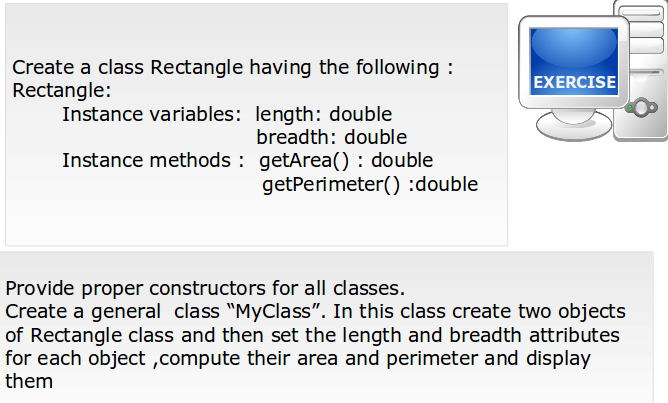
\includegraphics[scale=0.4]{COJ-M01-S05-Image1.png}
  \end{center}
\end{frame}
\begin{frame}{Encapsulation}
Access Modifiers
\begin{center}
        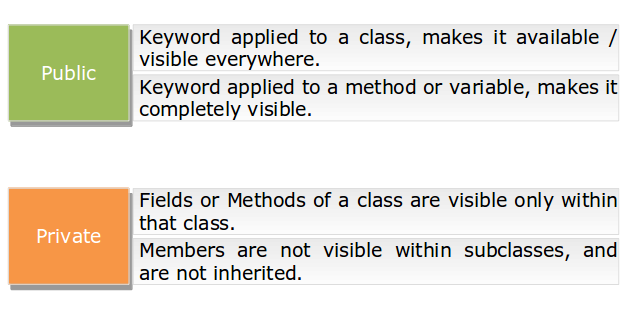
\includegraphics[scale=0.5]{COJ-M01-S05-Image2.png}
          \end{center}
      \end{frame}

      
\begin{frame}[fragile]{Encapsulation}
Visibility
\begin{lstlisting}[numbers=none]
class Rectangle {
    private double length;
    public breadth;
            // Constructor
    public Rectangle (double length, double breadth) {
        this. length = length;
	this. breadth = breadth;
    }
            //Methods to return circumference and area
    public double getPerimeter() {
        return 2* (length + breadth);
    }
    public double getArea() { 
        return length * breadth; 
    }	  
}
\end{lstlisting}
\end{frame}
\begin{frame}[fragile]{Encapsulation}
\begin{lstlisting}[numbers=none]
class MainClass {
    public static void main(String args[]){
        Rectngle rectangle1 = new Rectnagle(10,10);
	rectangle1. length = 10;   //  Error.  Private cannot be accessed  
                                        from out side the class
	rectangle1. breadth = 10;  // No Error.  public can be accessed from  
                                        outside the class.
        System.out.pritnln(rectangle1.getPerimeter());
	System.out.pritnln(rectangle1.getArea());
    }
}
\end{lstlisting}
\end{frame}
\begin{frame}{Encapsulation}
\begin{center}
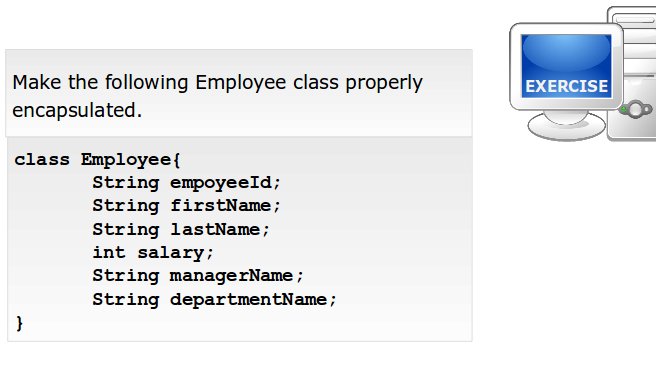
\includegraphics[scale=0.5]{COJ-M01-S05-Image3.png}
\end{center}
\end{frame}

\begin{frame}{Encapsulation}
\begin{center}
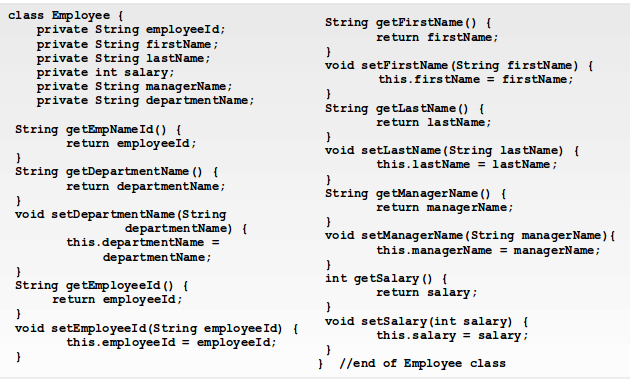
\includegraphics[scale=0.5]{COJ-M01-S05-Image4.png}
\end{center}
\end{frame}

\begin{frame}{Encapsulation}
\begin{block}{}
Encapsulation
\end{block}
\begin{itemize}
\item Encapsulation is the technique of making the fields in a class private and providing access to the fields via public methods.
\item If a field is declared private, it cannot be accessed by anyone outside the class, thereby hiding the fields within the class.
\item Encapsulation is also referred to as data hiding
\end{itemize}

\end{frame}


\begin{frame}{Encapsulation}
\begin{block}{}
Benefits of Encapsulation
\end{block}
\begin{itemize}
\item Ability to modify our implemented code without breaking the code of others who use our code.
\item Helps in protecting against accidental or wrong usage.
\item Gives maintainability, flexibility and extensibility to our code.
\end{itemize}

\end{frame}
\begin{frame}{Encapsulation}
\begin{center}

\includegraphics[scale=0.5]{COJ-M01-S05-Image5.png}
\end{center}
\end{frame}
\end{document}

